\section{Project Description}
\label{section:description}

The main contribution of this work should be to evaluate the boundaries of conventional machine learning approaches for hate speech detection. This includes manual feature extraction and subsequent text classification of doc\-u\-ments into hate speech and non-hate speech as opposed to modern deep learning approaches. Part of this work is also to find out which features and classifiers are suitable for such a classification task. The results should show which features work best for which classifier as well as which problems can be addressed with conventional machine learning methods and which not. A comparison to modern deep learning approaches should be drawn using the metrics of simple accuracy as well as precision and recall, respectively the F1-score. 

\begin{equation}
Accuracy = \frac{TP + TN}{TP + FP + TN + FN}
\end{equation}

\begin{equation}
Precision = \frac{TP}{TP + FP}
\end{equation}

\begin{equation}
Recall = \frac{TP}{TP + FN}
\end{equation}

\begin{equation}
F1-score = 2 \cdot \frac{Precision \cdot Recall}{Precision + Recall}
\end{equation}

The accuracy is used to measure how good a classifier can detect hate speech with the appropriate features while the F1-Score is used to evaluate how error-prone the chosen machine learning approach is. The F1-score is especially important as both used data sets are not class-balanced. As both data sets are annotated an automatic evaluation is possible. As a baseline, results of the mentioned papers as well as from papers documented in GitHub will be chosen. 

As stated above, the two data sets from \cite{ThomasDavidson.2020} and \cite{OnadeGibert.2020} will be used for this project. One possible problem could be that the amount of documents classified as pure hate speech in \cite{ThomasDavidson.2020} might not be enough to create profound classifiers. In this case one has to evaluate whether hate speech data from \cite{OnadeGibert.2020} is enough to achieve valid results or whether documents classified as offensive language from \cite{ThomasDavidson.2020} should be used as hate speech data as well. 

In \autoref{fig:pipeline} a schema of the project pipeline is shown. After having harmonized and consolidated the data sets into a common processable corpus one has to figure out which feature representations are commonly used in the area of hate speech detection and which classifiers are to be evaluated. This informationen will be based on the future lecture progress and further readings of the already introduced papers. The distribution of tasks can be done by feature-classifier combinations. In this sense the project can also be scaled without additional planning effort.  

\vspace{12pt}
To summarize the scope of the project the following subgoals were iden\-ti\-fied:

\begin{itemize}
	\item Prepare the data sets.
	\item Identify suitable feature representations and transform the data ac\-cord\-ingly.
	\item Identify and train machine learning classifiers.
	\item Combine classifiers with different feature representations.
	\item Evalute and compare the performance using accuracy, precision, recall and F1-score.
	\item Show the boundaries of conventional machine learning approaches in comparison to deep learning approaches.
\end{itemize}

The results of the project can contribute to offer an easier way to detect hate speech without having to train deep neural networks. It furthermore gives a more holistic view on different approaches to handle hate speech detection with conventional machine learning and text analytics methods and last but not least helps to fight hate speech on social media platforms.

\begin{figure}[t]
	\centering
	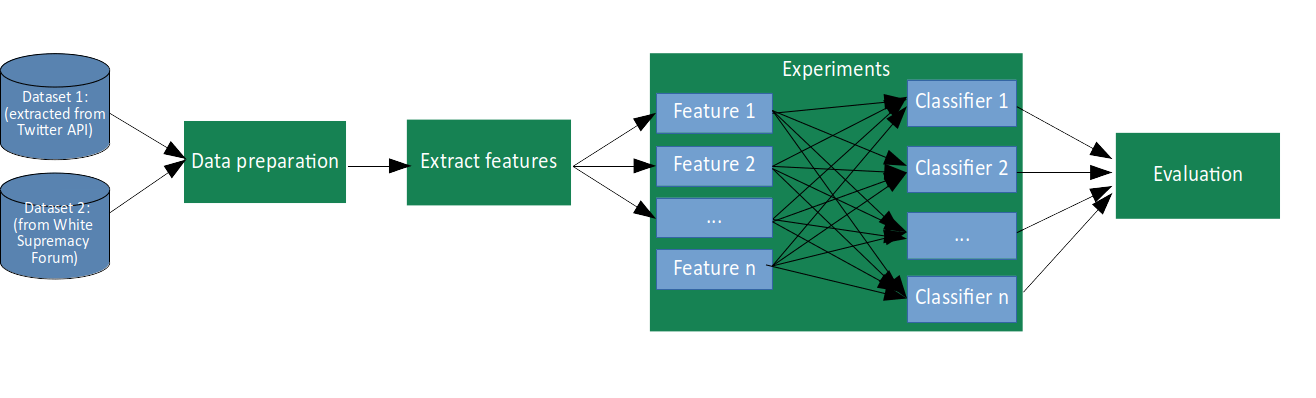
\includegraphics[width=1.0\textwidth]{./pipeline.png}	
	\caption{Text Analytics Pipeline}
	\label{fig:pipeline}
\end{figure}
